\section{Auswertung}
\label{sec:Auswertung}
Die in dieser Auswertung erstellten Plots werden mithilfe der \textit{Python}-Erweiterung 
\textit{matplotlib}~\cite{matplotlib} erstellt. Die Fortplanzung der Messunsicherheiten werden mithilfe von
\textit{uncertainties}~\cite{uncertainties} bestimmt und genügen der Gaußschen Fehlerfortpflanzung
\begin{equation}
    \symup{\Delta} F = \sqrt{\sum_{i}\left(\frac{\symup{d}F}{\symup{d}y_{i}}\symup{\Delta} y_{i} \right)^2}.
    \label{eq:Gauss}
\end{equation}
Die Messunsicherheiten der Zählraten $N$ sind poissonverteilt und werden daher mit $\symup{\Delta}N = \sqrt{N}$ berechnet.

\subsection{Charakteristik des GMZ}
Die Charakteristik des GMZ wird bestimmt, indem die Anzahl der pro Sekunde gemessenen Impulse in Abhängigkeit
von der anliegenden Zählrohrspannung aufgetragen wird. Hierbei lassen sich große Abweichungen einzelner Messwertgruppen
beobachten, die im Folgenden nicht weiter betrachet werden.\footnote{Anm.: Dies geschieht aufgrund einer bekannten Fehlfunktion
eines Verstärkers im Versuchsaufbau. Die Auswirkungen auf den weiteren Versuch werden in Abschnitt \ref{sec:Diskussion}
ausführlich diskutiert.}

\begin{longtable}{c c c c}
    \caption{Messwerte zur Bestimmung der Charakteristik des GMZ sowie der freigesetzten Ladung. Für den Strom $I$ wird eine %
    Messunsicherheit von $\symup{\Delta} I = \qty{0.1}{\micro\ampere}$ angenommen.} \label{tab:messdaten} \\
    \hline
    {$U \mathbin{/} \unit{\volt}$} & {Zählrate} & {$N \mathbin{/} {\unit{\second}}$} & {$I \mathbin{/} \unit{\micro\ampere}$} \\
    \hline
    \endfirsthead
    \caption[]{Messwerte zur Bestimmung der Charakteristik des GMZ sowie der freigesetzten Ladung. Für den Strom $I$ wird eine %
    Messunsicherheit von $\symup{\Delta} I = \qty{0.1}{\micro\ampere}$ angenommen.(Fortsetzung)}\\
    \hline
    {$U \mathbin{/} \unit{\volt}$} & {Zählrate} & {$N \mathbin{/} {\unit{\second}}$} & {$I \mathbin{/} \unit{\micro\ampere}$} \\
    \hline
    \endhead
    \hline
    \endfoot
    330 & $\num{ 9880+- 99}$ & $\num{ 82.33+-0.83}$ & 0,1 \\
    340 & $\num{ 9994+-100}$ & $\num{ 83.28+-0.83}$ & 0,2 \\
    350 & $\num{10221+-101}$ & $\num{ 85.17+-0.84}$ & 0,2 \\
    360 & $\num{10159+-101}$ & $\num{ 84.66+-0.84}$ & 0,2 \\
    370 & $\num{10393+-102}$ & $\num{ 86.61+-0.85}$ & 0,2 \\
    380 & $\num{10326+-102}$ & $\num{ 86.05+-0.85}$ & 0,2 \\
    390 & $\num{10443+-102}$ & $\num{ 87.03+-0.85}$ & 0,2 \\
    400 & $\num{10516+-103}$ & $\num{ 87.63+-0.85}$ & 0,3 \\
    410 & $\num{10457+-102}$ & $\num{ 87.14+-0.85}$ & 0,3 \\
    420 & $\num{10719+-104}$ & $\num{ 89.33+-0.86}$ & 0,4 \\
    430 & $\num{13720+-117}$ & $\num{114.33+-0.98}$ & 0,4 \\
    440 & $\num{16377+-128}$ & $\num{136.47+-1.07}$ & 0,4 \\
    450 & $\num{16365+-128}$ & $\num{136.38+-1.07}$ & 0,4 \\
    460 & $\num{15932+-126}$ & $\num{132.77+-1.05}$ & 0,4 \\
    470 & $\num{14108+-119}$ & $\num{117.57+-0.99}$ & 0,4 \\
    480 & $\num{10787+-104}$ & $\num{ 89.89+-0.87}$ & 0,5 \\
    490 & $\num{10606+-103}$ & $\num{ 88.38+-0.86}$ & 0,5 \\
    500 & $\num{10553+-103}$ & $\num{ 87.94+-0.86}$ & 0,5 \\
    510 & $\num{10562+-103}$ & $\num{ 88.02+-0.86}$ & 0,5 \\
    520 & $\num{10617+-103}$ & $\num{ 88.47+-0.86}$ & 0,6 \\
    530 & $\num{10990+-105}$ & $\num{ 91.58+-0.87}$ & 0,6 \\
    540 & $\num{12046+-110}$ & $\num{100.38+-0.91}$ & 0,6 \\
    550 & $\num{13559+-116}$ & $\num{112.99+-0.97}$ & 0,6 \\
    560 & $\num{13181+-115}$ & $\num{109.84+-0.96}$ & 0,6 \\
    570 & $\num{10699+-103}$ & $\num{ 89.16+-0.86}$ & 0,6 \\
    580 & $\num{10575+-103}$ & $\num{ 88.12+-0.86}$ & 0,6 \\
    590 & $\num{10779+-104}$ & $\num{ 89.83+-0.87}$ & 0,6 \\
    600 & $\num{10668+-103}$ & $\num{ 88.90+-0.86}$ & 0,7 \\
    610 & $\num{10622+-103}$ & $\num{ 88.52+-0.86}$ & 0,7 \\
    620 & $\num{10611+-103}$ & $\num{ 88.42+-0.86}$ & 0,7 \\
    630 & $\num{10858+-104}$ & $\num{ 90.48+-0.87}$ & 0,7 \\
    640 & $\num{10640+-103}$ & $\num{ 88.67+-0.86}$ & 0,7 \\
    650 & $\num{10761+-104}$ & $\num{ 89.67+-0.86}$ & 0,7 \\
    660 & $\num{10878+-104}$ & $\num{ 90.65+-0.87}$ & 0,8 \\
    670 & $\num{10774+-104}$ & $\num{ 89.78+-0.86}$ & 0,8 \\
    680 & $\num{10727+-104}$ & $\num{ 89.39+-0.86}$ & 0,8 \\
    690 & $\num{11005+-105}$ & $\num{ 91.71+-0.87}$ & 0,8 \\
    700 & $\num{11160+-106}$ & $\num{ 93.00+-0.88}$ & 0,8 \\
    \bottomrule
\end{longtable}

\begin{figure}[H]
    \centering
    \includegraphics[height=8cm]{build/charakteristik_roh.pdf}
    \caption{Graphische Darstellung der Messwerte zur Bestimmung der Charakteristik des GMZ aus%
    \autoref{tab:messdaten}.}
    \label{fig:charakteristik_roh}
\end{figure}

\begin{figure}[H]
    \centering
    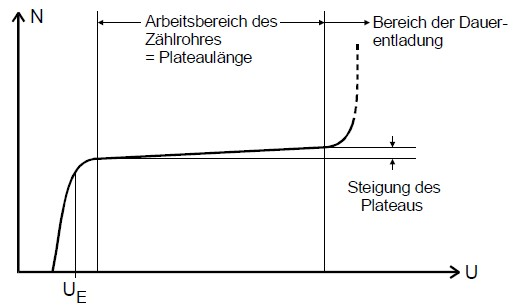
\includegraphics[height=8cm]{build/charakteristik.pdf}
    \caption{Graphische Darstellung der Charakteristik des GMZ mit eingezeichneter Ausgleichsgerade der %
    Messwerte des Plateaus. Die in \autoref{fig:charakteristik_roh} gekennzeichneten stark abweichenden %
    Messwerte werden hierbei nicht berücksichtigt.}
    \label{fig:charakteristik}
\end{figure}

In \autoref{fig:charakteristik} ist ein Bereich auszumachen, in dem die Anzahl der Impulse annähernd linear
zunimmt. Dieser Bereich wird auch Plateaubereich genannt und hat eine Länge von $L=\qty{290}{\volt}$. Mithilfe der \textit{Python}-Erweiterung \textit{scipy} \cite{scipy} wird eine lineare Ausgleichsrechnung
für die Werte in dem Plateaubereich durchführt. Für eine Ausgleichsgerade des Typs $y=mx + b$ ergeben sich die
Werte
\begin{align*}
    m_{\text{Regression}} &= \qty{0.0070+-0.0019}{\per\second\per\volt} & b &= \qty{85.0+-1.0}{\per\second}.
\end{align*}

Die Plateausteigung wird üblicher Weise in der Einheit $\frac{1\,\%}{100\,V}$ angegeben. Dafür wird die Steigung aus der Regression mit 100 multipliziert 
und durch den ungefähren Wert der Plateaumitte dividiert
\begin{equation*}
    m_{\text{Plateau}} = \frac{100 m_{\text{Regression}}}{N_{\text{Mitte}}}.
\end{equation*}

Für die Messunsicherheit der Plateausteigung folgt nach der Gaußschen Fehlerfortpflanzung~\eqref{eq:Gauss}

\begin{align*}
    \symup{\Delta}m_{\text{Plateau}} &= \sqrt{\left(\frac{\symup{d}m_{\text{Plateau}}}{\symup{d}m_{\text{Regression}}}\symup{\Delta} m_{\text{Regression}} \right)^2 + %
     \left(\frac{\symup{d}m_{\text{Plateau}}}{\symup{d}N_{\text{Mitte}}}\symup{\Delta} N_{\text{Mitte}} \right)^2} \\
     &=\sqrt{\left(\frac{100}{N_{\text{Mitte}}}\symup{\Delta} m_{\text{Regression}}\right)^2 + \left(\frac{100 m_{\text{Regression}}}{N_{\text{Mitte}}^2}\symup{\Delta} N_{\text{Mitte}}\right)^2}.
\end{align*}

Die Zählrate bei der ungefähren Plateaumitte bei $U_{\text{Mitte}}\approx \qty{550}{\volt}$ wird zu $N_{\text{Mitte}} \approx \qty{89}{\per\second}$
bestimmt. Somit folgt für die Plateausteigung
\begin{equation*}
    m_{\text{Plateau}} = \qty{0.78+-0.21}{\percent\per100\volt}.
\end{equation*}

\subsection{Bestimmung der Totzeit mit einem Oszilloskop}
Die Totzeit des GMZ wird zunächst mithilfe eines Oszilloskops, das an das GMZ angeschlossen ist, bestimmt. In \autoref{fig:Nachentladung} 
ist ein entsprechendes Bild zu sehen.\footnote{Anm.: Hierbei wird auf Daten unserer Parallelgruppe zurückgeriffen, sodass hier ein 
anderes GMZ als in dem ersten Teil des Versuches verwendet wird. Dies hat den Grund, dass die zuerst aufgenommenen Daten aufgrund der bekannten
Fehlfunktion des Verstärkers unzulänglich sind.} Die Totzeit des GMZ ist der Abstand zwischen dem Hauptpeak und der Stelle, wo die Amplitude wieder auf 
Null abgesunken ist. Es wird eine Totzeit von
\begin{equation*}
    T_{\text{Oszilloskop}} \approx \qty{100}{\micro\second}
\end{equation*}
abegelesen.

Neben der Totzeit lässt sich aus \autoref{fig:Nachentladung} auch die Zeit zwischen Primär- und Nachentladungsimpulsen. Dieser ergibt sich als Abstand
zwischen dem Maximum des Hauptpeaks und dem Maximum des ersten Sekundärpeaks und wird zu $\qty{120}{\micro\second}$ bestimmt.

\begin{figure}[H]
    \centering
    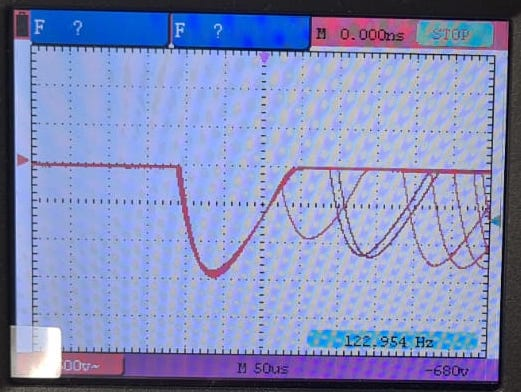
\includegraphics[height=7cm]{content/pics/Nachentladung.jpg}
    \caption{Bild des Displays des Oszilloskops zur Bestimmung der Totzeit des GMZ. 1 Kästchen entspricht $\qty{50}{\micro\second}$.}
    \label{fig:Nachentladung}
\end{figure}

\subsection{Bestimmung der Totzeit über die Zwei-Quellen-Methode}
Die Totzeit des GMZ lässt sich auch über die in Abschnitt \ref{sec:Totzeit} beschriebene \textit{Zwei-Quellen-Methode} berechnen. Eine Darstellung
der Messdaten ist in \autoref{tab:Totzeit} gegeben.\footnote{Anm.: Hierbei wird erneut aus dem bereits beschriebenen Grund auf die Daten 
unserer Parallelgruppe zurückgeriffen.}
\begin{table}[H]
    \centering
    \caption{Darstellung der Messwerte zur Bestimmung der Totzeit über die \textit{Zwei-Quellen-Methode}. Die Messdauer beträgt 120\,s.}
    \label{tab:Totzeit}
    \begin{tabular}{c S S}
      \toprule
      {Strahler} & {Zählrate} & {$N \mathbin{/} {\unit{\second}}$}\\
      \midrule
      $1$   & $\num{19706+-140}$ & $\num{164.2+-1.2}$ \\
      $2$   & $\num{34902+-187}$ & $\num{290.9+-1.6}$ \\
      {1 und 2} & $\num{15897+-126}$ & $\num{132.5+-1.1}$ \\
      \bottomrule
    \end{tabular}
  \end{table}
Über den Zusammenhang \eqref{eq:2 Quellen} wird die Totzeit berechnet, wobei sich hier die Unsicherheit über die Gaußsche 
Fehlerfortpflanzung~\eqref{eq:Gauss}
\begin{align*}
    \symup{\Delta}T_{\text{2-Quellen}} 
    &= \sqrt{\left(\frac{\symup{d}T_{\text{2-Quellen}}}{\symup{d}N_1}\symup{\Delta} N_1 \right)^2 
    + \left(\frac{\symup{d}T_{\text{2-Quellen}}}{\symup{d}N_2}\symup{\Delta} N_2 \right)^2
    + \left(\frac{\symup{d}T_{\text{2-Quellen}}}{\symup{d}N_{1,2}}\symup{\Delta} N_{1,2} \right)^2} \\
    &= \sqrt{\left(\frac{N_1 - N_{1,2}}{2N_2 N_1^2} \cdot \symup{\Delta}N_1 \right)^2 
    + \left(\frac{N_{1,2} - N_{1}}{2N_1 N_2^2} \cdot \symup{\Delta}N_2 \right)^2
    + \left( \frac{1}{2N_1 N_2}\symup{\Delta}N_{1,2}\right)^2}
\end{align*}
bestimmt.
Die Totzeit ergibt sich so zu
\begin{equation*}
    T_{\text{2-Quellen}} = \qty{130+-50}{\micro\second}.
\end{equation*}

\subsection{Freigesetzte Ladung im GMZ}
Die freigesetzte Ladungsmenge lässt sich bestimmen, indem die Formel \eqref{eq:strom} umgestellt wird und für die 
Zählrate~$N=\frac{Z}{120\,s}$ und $t=120\,s$ eingesetzt werden. Es folgt
\begin{equation*}
    Q = \frac{\bar{I}}{N}.
\end{equation*}
Die Unsicherheit der freigesetzten Ladungsmenge beträgt
\begin{align*}
    \symup{\Delta}Q &= \sqrt{\left(\frac{\symup{d}Q}{\symup{d}\bar{I}}\symup{\Delta} \bar{I} \right)^2
    + \left(\frac{\symup{d}Q}{\symup{d}N}\symup{\Delta} N \right)^2} \\
    &= \sqrt{\left(\frac{1}{N}\symup{\Delta} \bar{I}\right)^2 + \left(\frac{I}{N^2} \symup{\Delta} N\right)^2}.
\end{align*}
Werden die gemessenen Ströme und Impulse aus \autoref{tab:messdaten} in diesen Zusammenhang eingesetzt, ergeben sich die dabei freigesetzten Ladungsmengen.
Diese sind in \autoref{tab:Ladungen} dargestellt und werden außerdem in \autoref{fig:ladung} graphisch veranschaulicht. 
Es ist zu erkennen, dass die freigesetzte Ladungsmenge annähernd proportional zu dem gemessenen Strom steigt.
\begin{figure}[H]
    \centering
    \includegraphics[height=8cm]{build/ladung.pdf}
    \caption{Darstellung der freigesetzten Ladungen in Abhängikeit von den gemessenen Strömen mit eingezeichneter 
    Ausgleichsgeraden. Die Unsicherheiten des Strom sind konstant und betragen $\symup{\Delta} I = \qty{0.1}{\micro\ampere}$.}
    \label{fig:ladung}
\end{figure}